\documentclass{beamer}

\usepackage{minted}
\usepackage{booktabs}

\usetheme{Madrid}
\useoutertheme{miniframes}
\useinnertheme{circles}

\definecolor{BGUorange}{RGB}{247, 148, 30}
\definecolor{BGUgrey}{RGB}{88, 89, 91}

\setbeamercolor{palette primary}{bg=BGUorange,fg=white}
\setbeamercolor{palette secondary}{bg=BGUorange,fg=white}
\setbeamercolor{palette tertiary}{bg=BGUorange,fg=white}
\setbeamercolor{palette quaternary}{bg=BGUorange,fg=white}
\setbeamercolor{structure}{fg=BGUorange} % itemize, enumerate, etc
\setbeamercolor{section in toc}{fg=BGUorange} % TOC sections

% Override palette coloring with secondary
\setbeamercolor{subsection in head/foot}{bg=BGUgrey,fg=white}


\title[CS PhD Seminar]{Text-to-SQL Parsing: Using Execution Plans as an Intermediate Language}
\author{Ben Eyal}
\date{January 3rd, 2024}

\titlegraphic{
\includegraphics[height=1cm]{eng-logo.png}\hfill~
\includegraphics[height=1cm]{bgunlplogo.jpg}}

\AtBeginSection[]{
  \begin{frame}
    \frametitle{Table of Contents}
    \tableofcontents[currentsection]
  \end{frame}
}

\begin{document}
\beamertemplatenavigationsymbolsempty

\begin{frame}
    \titlepage
\end{frame}

\section{Introduction \& Motivation}

\begin{frame}{What is ``Understanding''?}
    \begin{itemize}
        \item Let's address the elephant in the room: does ChatGPT \alert{understand} us?\footnote{ChatGPT or any of the Large Language Models (LLMs) that have appeared in the past two years - Llama, Gemini, Claude...}
        
        \pause
        
        \item On the one hand, it's only a language model: it predicts the next word given the previous ones. It can't possibly understand!
        
        \pause
        
        \item On the other hand...
    \end{itemize}
\end{frame}

\begin{frame}{What is ``Understanding''?}
    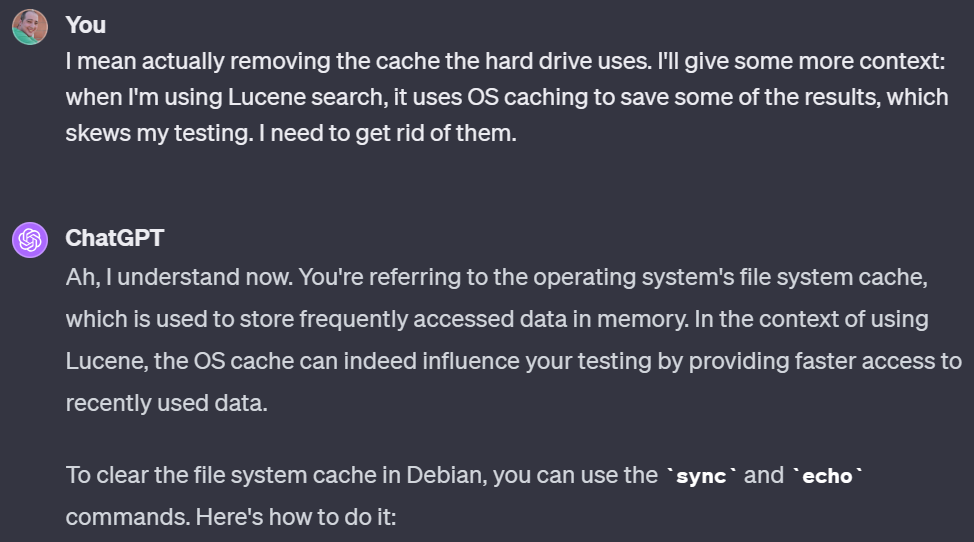
\includegraphics[width=\textwidth]{chatgpt_convo_1.png}
\end{frame}

\begin{frame}{What is ``Understanding''?}
    \begin{itemize}
        \item Although sometimes...
    \end{itemize}
\end{frame}

\begin{frame}{What is ``Understanding''?}
    \begin{figure}
        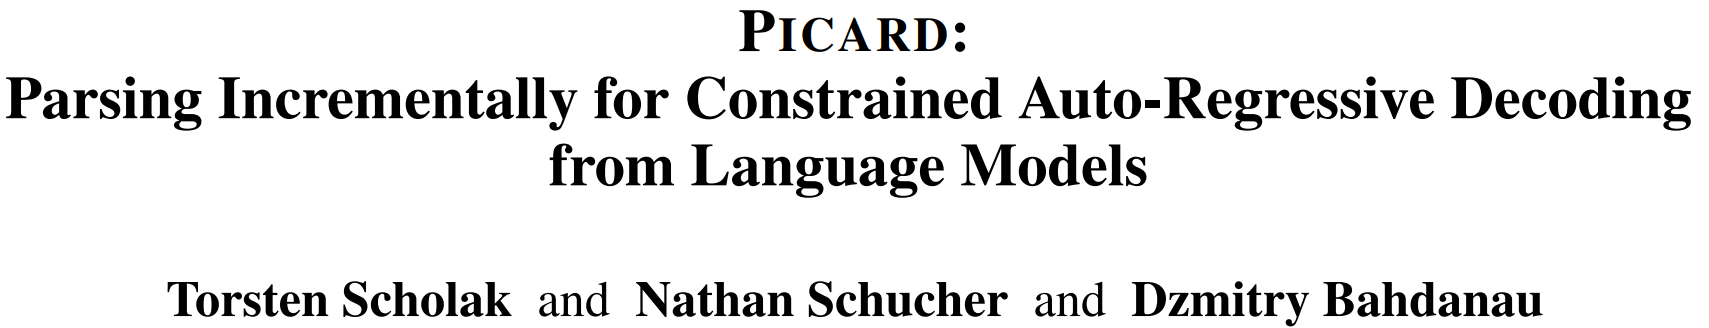
\includegraphics[width=\textwidth]{picard_title.png}
    \end{figure}

    \begin{figure}
        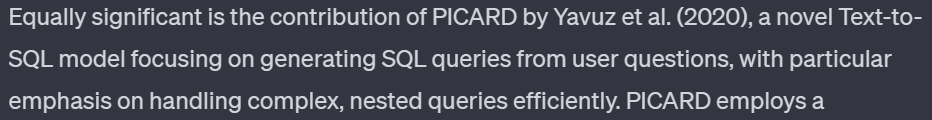
\includegraphics[width=\textwidth]{yavuzetal.png}
    \end{figure}
\end{frame}

\begin{frame}{Assessing a Model's Language Understanding}
    \begin{itemize}
        \item The observed executions of LLMs mix apparent understanding with overconfident \alert{hallucinations}
        \item We don't know how to define ``understand'' as a binary predicate that can be verified.

        \pause

        \item Task-oriented benchmarks to the rescue!
    \end{itemize}
\end{frame}

\begin{frame}{Assessing a Model's Language Understanding}
    \begin{figure}
        \centering
        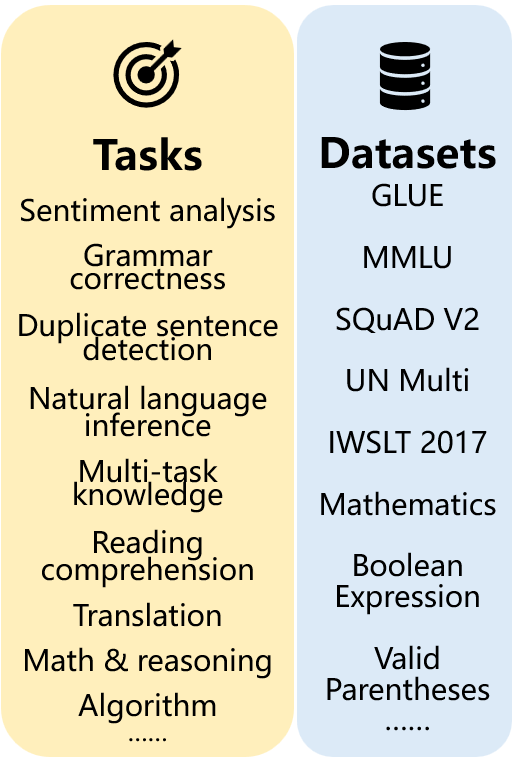
\includegraphics[height=0.8\textheight]{promptbench_2.png}
    \end{figure}
\end{frame}

\begin{frame}{Assessing a Model's Language Understanding}
    \begin{itemize}
        \item In addition to measuring understanding on various \textbf{tasks} and various \textbf{domains} (similar to \alert{test cases})
        \item We also want to verify that the model behavior satisfies expected properties of understanding (similar to \alert{property-based testing})
        \item Two approaches:
            \begin{itemize}
                \item Consistency testing (model should not say $p$ and $\neg p$)
                \item Compositionality
            \end{itemize}
    \end{itemize}
\end{frame}

\begin{frame}{Compositionality}
    \begin{itemize}
        \item Principle that the meaning of a \textbf{complex expression} is determined by the \textbf{meanings of its constituent expressions} and the \textbf{rules used to combine them}. 
        \item If a model can interpret simple expressions, it should be able to interpret their syntactic combination.
    \end{itemize}
\end{frame}

\begin{frame}{Measuring Compositionality - Specialized Benchmarks}
    \begin{figure}
        \centering
        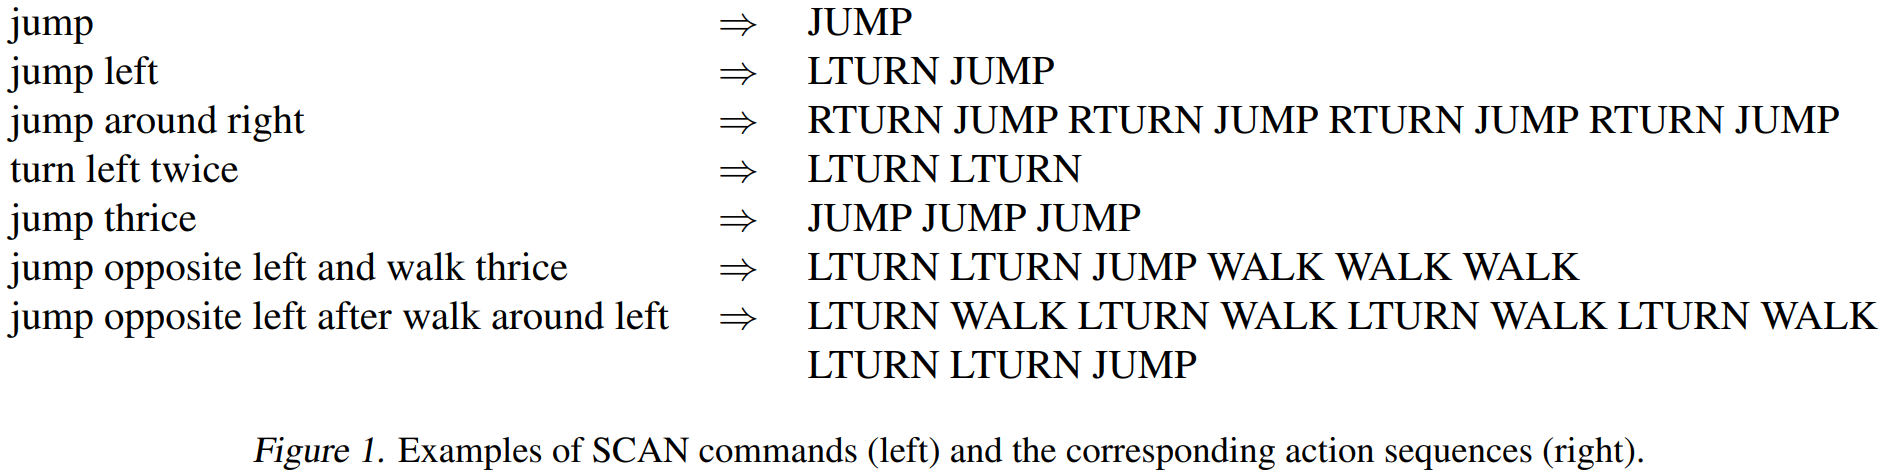
\includegraphics[width=\textwidth]{scan.png}
    \end{figure}
    \begin{itemize}
        \item SCAN: Synthetic benchmark based on a simple grammar
        \item Measure models capability to parse complex expressions\\(Depth and syntactic structure unseen at training time).
    \end{itemize}

    \vfill
    
    \tiny{Source: B. Lake \& M. Baroni, \emph{Generalization without Systematicity: On the Compositional Skills of Sequence-to-Sequence Recurrent Networks}, 2018}\\
    \tiny{Kim and Linzen, \textit{COGS: A Compositional Generalization Challenge Based on Semantic Interpretation}, EMNLP 2020}
\end{frame}

\begin{frame}{Measuring Compositionality - Compositional Splits}
    \begin{figure}
        \centering
        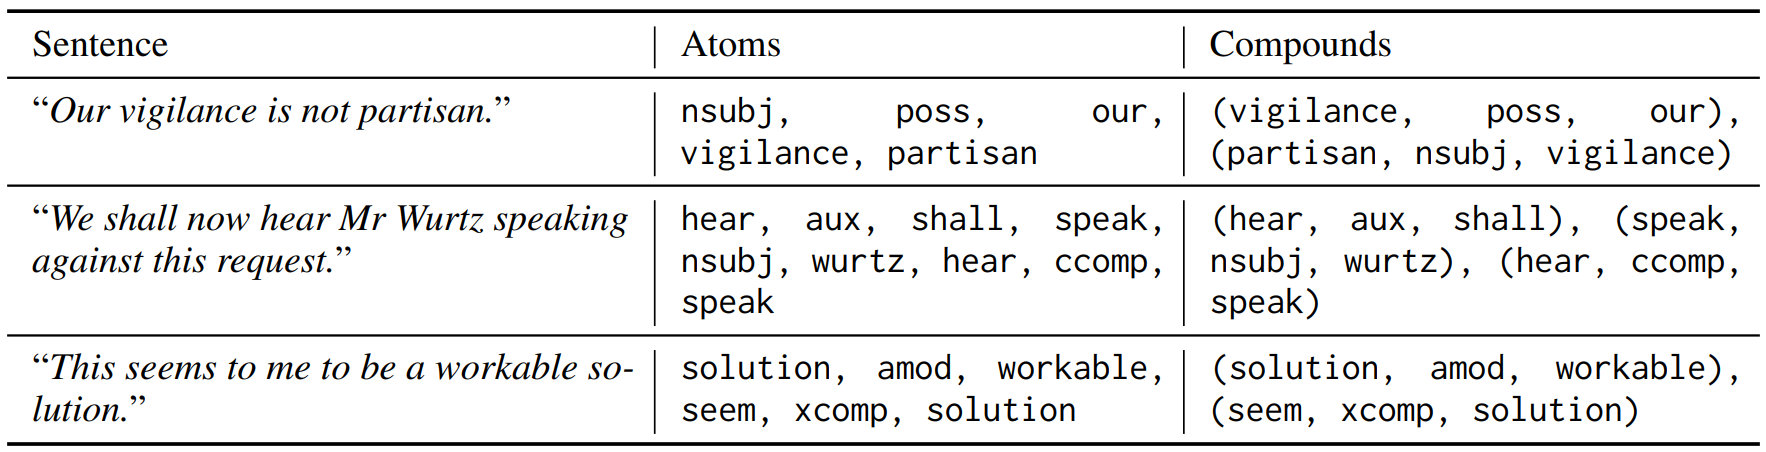
\includegraphics[width=\textwidth]{dbca.png}
    \end{figure}
    \begin{itemize}
        \item Distinguish generalization on lexical items and on syntactic structure.
        \item Split the training/test datasets so that the distributions of compound expressions are as different as possible.
    \end{itemize}

    \vfill

    \tiny{D. Keysers et al., \emph{Measuring Compositional Generalization: A Comprehensive Method on Realistic Data}, ICLR 2020}
    
    \tiny{A. Moisio, M. Creutz, and M. Kurimo, \emph{On Using Distribution-Based Compositionality Assessment to Evaluate Compositional Generalisation in Machine Translation}, GenBench 2023}
\end{frame}

\begin{frame}{Research Question 1}
    \begin{center}
        How do we assess compositional generalization\\on complex / realistic tasks?
    \end{center}
\end{frame}

\begin{frame}{Semantic Parsing}
    \begin{itemize}
        \item Translate natural language to a logical form.

        \pause

        \item Some logical forms can be executed to produce a denotation.

        \pause

        \item For example: $\lambda$-calculus, SQL, Python, etc.
    \end{itemize}
\end{frame}

\begin{frame}{Semantic Parsing vs. Question Answering}
    \begin{itemize}
        \item Why bother with semantic parsing? We have QA!

        \begin{itemize}
            \item SP: Question $\rightarrow$ Logical Form $\rightarrow$ Answer
            \item QA: Question $\rightarrow$ Answer
        \end{itemize}

        \pause

        \item QA is a ``uniform format'' to interact with NLP systems.
        
        \pause
        
        \item QA is universal - it tests linguistic capabilities as well as world knowledge in any domain.
        
        \pause
        
        \item Any task can be ``reduced'' to a QA task.
    \end{itemize}
\end{frame}

\begin{frame}{Semantic Parsing vs. Question Answering}
    \begin{itemize}
        \item QA is hard to assess!

        \pause

        \item Different questions can lead to the same answer (variability), the same question to different answers (ambiguity).

        \pause

        \item Hard to compare predicted answer with expected one!

        \pause

        \item QA learns \textbf{what} to answer, SP learns \textbf{how} to answer and can use complicated skills that are hard to learn (e.g., arithmetic).
    \end{itemize}
\end{frame}

\begin{frame}{Semantic Parsing vs. Question Answering}
    \begin{itemize}
        \item In SP we have known semantics for the logical form, so we can probe semantic properties of the predicted logical form.

        \pause

        \item In text-to-code, if the expected and predicted snippets run and produce the same denotation, we know the semantic parser is fine.

        \pause

        \item The predicted logical form is a form of ``explanation'' of what was understood by the parser - it can be probed by humans.
    \end{itemize}
\end{frame}

\begin{frame}{Research Question 2}
    \begin{center}
        Do humans benefit from generated code to verify that the answer generated by the semantic parser is a reliable answer to the question?
    \end{center}
\end{frame}

\begin{frame}{The Text-to-SQL Task}
    \begin{itemize}
        \item SQL is the de-facto language for interacting with relational databases
        \item For non-expert users, SQL can be daunting for any non-trivial query
        \item Text-to-SQL models can help alleviate the pain points of crafting an SQL query by hand by ``translating'' a question in natural language and a database schema to a corresponding SQL query
        \item Many datasets for this task, most prominent in the past few years being ``Spider'', a cross-domain dataset of questions, schemas and queries
    \end{itemize}

    \vfill

    \tiny{Yu et al., \emph{Spider: A Large-Scale Human-Labeled Dataset for Complex and Cross-Domain Semantic Parsing and Text-to-SQL Task}, EMNLP 2018}
\end{frame}

\begin{frame}[fragile]{Spider Example}
    Question: What is the number of cars with more than 4 cylinders?\\

    Schema:
    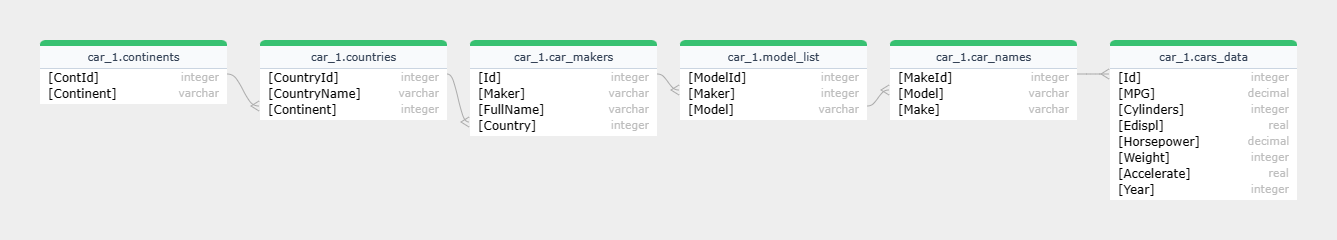
\includegraphics[width=\textwidth]{car_1_erd.png}

    SQL:
    \begin{minted}{sql}
    SELECT COUNT(*)
    FROM cars_data
    WHERE cylinders > 4
    \end{minted}
\end{frame}

\begin{frame}{Spider Dataset}
    \begin{itemize}
        \item Spider's training and development schema are disjoint, i.e, models cannot rely on previous schema knowledge during inference
        \item 7,000 training examples and 1,034 development examples spanning 166 different schemas and 874 tables
        \item Divided into four difficulty levels: easy, medium, hard, and extra-hard
        \item Distribution of training examples by difficulty level:
        \begin{itemize}
            \item 24\% Easy
            \item 40\% Medium
            \item 21\% Hard
            \item 15\% Extra-hard
        \end{itemize}
    \end{itemize}
\end{frame}

\begin{frame}{Research Questions}
    \begin{itemize}
        \item[RQ1] How do we assess and improve compositional generalization of text-to-SQL?

        \item[RQ2] Do people benefit from the generated code to assess the reliability of answers produced by text-to-SQL (considered as a QA system producing answers)?

        \item[RQ3] How robust are models to variations in question formulation - in particular on schema linking - in a multilingual setting?
    \end{itemize}
\end{frame}

\section{Challenges}

\begin{frame}[fragile]{SQL Syntax is Problematic}
    \begin{itemize}
        \item The \alert{syntactical} order does not match the \alert{logical} order, e.g., \texttt{SELECT} is (usually) the last operation that happens on the result, yet it is the first token in an SQL query

        \item IDEs can't help with SQL autocompletion before specifying the \texttt{FROM} clause

        \begin{minted}[fontsize=\scriptsize]{sql}
        -- Don't you wish this would be completed to first_name?
        SELECT first_na...
 
        -- Aaah, now it works:
        SELECT first_na...
        FROM customer
        \end{minted}
        
        \item \texttt{GROUP BY} (and aggregations in general) is confusing w.r.t order of operations, i.e., whether an aggregation has already happened or not is not always clear \alert{syntactically}
    \end{itemize}

    \vfill

    \tiny{See: ``A Beginner's Guide to the True Order of SQL Operations'' by Lukas Eder}
\end{frame}

\begin{frame}{Complex Queries are Hard for People to Understand}
    User experiment: 
    \begin{itemize}
        \item 10 (question, complex SQL query) pairs shown to 4 programmers
        \item half are correct and half incorrect. 
    \end{itemize}
    
    how often programmers were right in assessing the correctness of the query?
    
    \begin{table}[h]
    \centering
    \begin{tabular}{lc}
        \toprule
        \textbf{Gold label} & \textbf{Correctness of Judgment} \\
        \midrule
        Incorrect query & 50\% \\
        Correct query   & 25\% \\
        \bottomrule
    \end{tabular}
    \end{table}
\end{frame}

\begin{frame}{Complex Queries are Hard for Models to Learn}

\begin{table}[h]
\centering
\begin{tabular}{lccc}
\toprule
Difficulty & NatSQL + RAT-SQL & Din-SQL GPT-4 & GPT3.5-turbo\\
\midrule
Easy       & 91.6\% & 91.1\% & 87.7\% \\
Medium     & 75.2\% & 79.8\% & 75.1\% \\
Hard       & 65.5\% & 64.9\% & 72.5\% \\
Extra Hard & \alert{51.8\%} & \alert{43.4\%} & \alert{53.9\%} \\
\midrule
Overall & 73.7\% & 74.2\% & 74.3\% \\
\bottomrule
\end{tabular}
\end{table}
\end{frame}

% \begin{frame}{Research Questions}
%     \begin{enumerate}
%         \item How to deal with questions associated to complex SQL queries?
%         \item Will a compositional data retrieval language be easier to learn and lead to better generalization for complex queries than SQL?
%     \end{enumerate}
% \end{frame}

\section{Method}

\begin{frame}{Approach}
\begin{enumerate}
    \item Define QPL - a new data retrieval language:
    \begin{itemize}
        \item Modular
        \item Executable
        \item Regular
    \end{itemize}
    
    \item Automatically translate the Spider dataset from SQL to QPL 

    \item Compare training the same neural architecture on (Q $\rightarrow$ SQL) and\\ (Q $\rightarrow$ QPL).
\end{enumerate}
    
\end{frame}

\begin{frame}{SQL Execution Plans}
    Starting Point: SQL Optimizer
    \begin{itemize}
        \item When a database engine is given a query, it must construct a ``plan''
        \item A ``plan'' is a DAG of operations on streams of rows
        \item This DAG is then optimized to give the fastest performing execution of the query
    \end{itemize}
\end{frame}

\begin{frame}[fragile]{SQL Execution Plans}
    For example, for the following query:

    \begin{minted}[fontsize=\footnotesize]{SQL}
                SELECT Theme, AVG(Age)
                FROM singer AS T1
                    JOIN singer_in_concert AS T2
                	ON T1.Singer_ID = T2.Singer_ID
                    JOIN concert AS T3
                        ON T2.concert_ID = T3.concert_ID
                GROUP BY Theme
    \end{minted}

    \vfill

    Microsoft SQL Server will produce the following plan:\\

    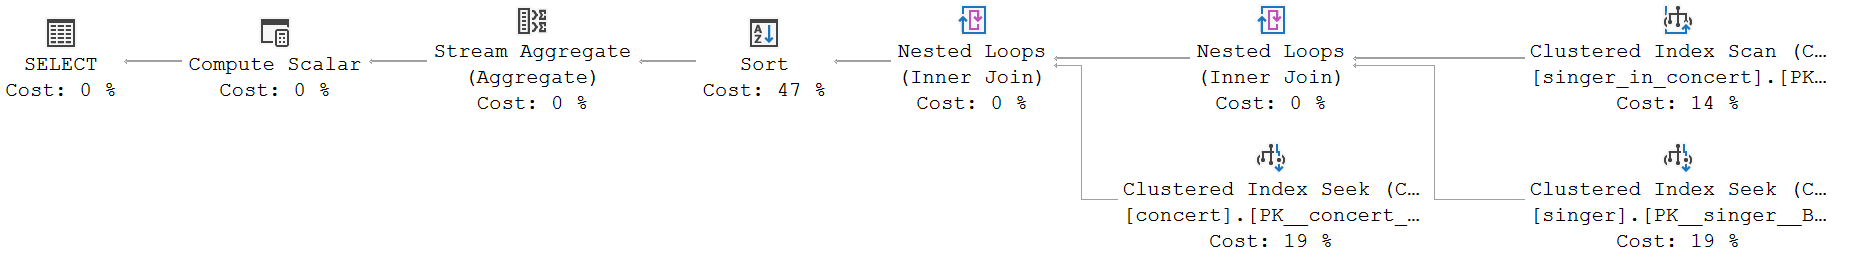
\includegraphics[width=\textwidth]{exec-plan.png}
\end{frame}

\begin{frame}{Query Plan Language}
    \begin{itemize}
        \item What if instead of mentally parsing an SQL query to understand what it does and at what point, we could read and write the query step-by-step?
        \item We introduce Query Plan Language (QPL), an intermediate language based on execution plans, that does just that
        \item The transformation from SQL to QPL is semantic instead of syntactic (NatSQL, Gan et al. 2021)
    \end{itemize}
\end{frame}

\begin{frame}[fragile]{Query Plan Language}
    For the earlier query, we get the following QPL:

    \begin{minted}[fontsize=\footnotesize]{sql}
#1 = Scan Table [ singer_in_concert ] Output [ concert_ID , Singer_ID ]
          
#2 = Scan Table [ singer ] Output [ Singer_ID , Age ]
          
#3 = Join [ #1 , #2 ] Predicate [ #1.Singer_ID = #2.Singer_ID ]
                      Output [ Age , concert_ID ]
                      
#4 = Scan Table [ concert ] Output [ concert_ID , Theme ]
          
#5 = Join [ #3 , #4 ] Predicate [ #3.concert_ID = #4.concert_ID ]
                      Output [ Age , Theme ]
                      
#6 = Aggregate [ #5 ] GroupBy [ Theme ]
                      Output [ AVG(Age) AS Avg_Age , Theme ]
    \end{minted}
\end{frame}

% @@@ Add a slide showing tree structure of QPL
% @@@ With a diagram

\begin{frame}{Query Plan Language Operators}
    \begin{table}[h]
  \centering
  \begin{tabular}{ll}
    \toprule
    \textbf{Operator} & \textbf{Description} \\
    \midrule
    \textbf{Aggregate} & Aggregate a stream of tuples into a stream of groups \\
    \textbf{Except} & Set difference between two streams of tuples \\
    \textbf{Filter} & Remove tuples from a stream that do not match a predicate \\
    \textbf{Intersect} & Intersection between two streams of tuples \\
    \textbf{Join} & Logical join  between two streams based on a join condition \\
    \textbf{Scan} & Scan all rows in a table with optional filtering predicate \\
    \textbf{Sort} & Sort a stream according to a sorting expression \\
    \textbf{TopSort} & Top-K tuples from a stream according to sort expr. \\
    \textbf{Union} & Set union between two streams of tuples \\
    \bottomrule
  \end{tabular}
\end{table}
\end{frame}

\begin{frame}[fragile]{Common Table Expression}
    Let's convert the following QPL to executable SQL:

    \begin{minted}[fontsize=\footnotesize]{sql}
#1 = Scan Table [ singer_in_concert ] Output [ concert_ID , Singer_ID ]
          
#2 = Scan Table [ singer ] Output [ Singer_ID , Age ]
          
#3 = Join [ #1 , #2 ] Predicate [ #1.Singer_ID = #2.Singer_ID ]
                      Output [ Age , concert_ID ]
                      
#4 = Scan Table [ concert ] Output [ concert_ID , Theme ]
          
#5 = Join [ #3 , #4 ] Predicate [ #3.concert_ID = #4.concert_ID ]
                      Output [ Age , Theme ]
                      
#6 = Aggregate [ #5 ] GroupBy [ Theme ]
                      Output [ AVG(Age) AS Avg_Age , Theme ]
    \end{minted}
\end{frame}

\begin{frame}[fragile]{Common Table Expression (CTE)}
    A ``common table expression'' (CTE) is a way to give names to intermediary results in an SQL query. The CTE for the above QPL is:

    \begin{minted}[fontsize=\footnotesize]{sql}
    WITH
    Scan_1 AS (SELECT concert_ID, Singer_ID FROM singer_in_concert),
    Scan_2 AS (SELECT Singer_ID, Age FROM singer),
    Join_3 AS (SELECT Age, concert_ID FROM Scan_1 JOIN Scan_2
               ON Scan_1.Singer_ID = Scan_2.Singer_ID),
    Scan_4 AS (SELECT concert_ID, Theme FROM concert),
    Join_5 AS (SELECT Age, Theme FROM Join_3 JOIN Scan_4
               ON Join_3.concert_ID = Scan_4.concert_ID),
    Aggregate_6 AS (SELECT AVG(Age) AS Avg_Age, Theme FROM Join_5
                    GROUP BY Theme)
    SELECT * FROM Aggregate_6
    \end{minted}

    This CTE is \alert{semantically equivalent} to the original complex SQL query.
\end{frame}

\begin{frame}{Spider $\rightarrow$ QPL Dataset Preparation}
    \begin{center}
        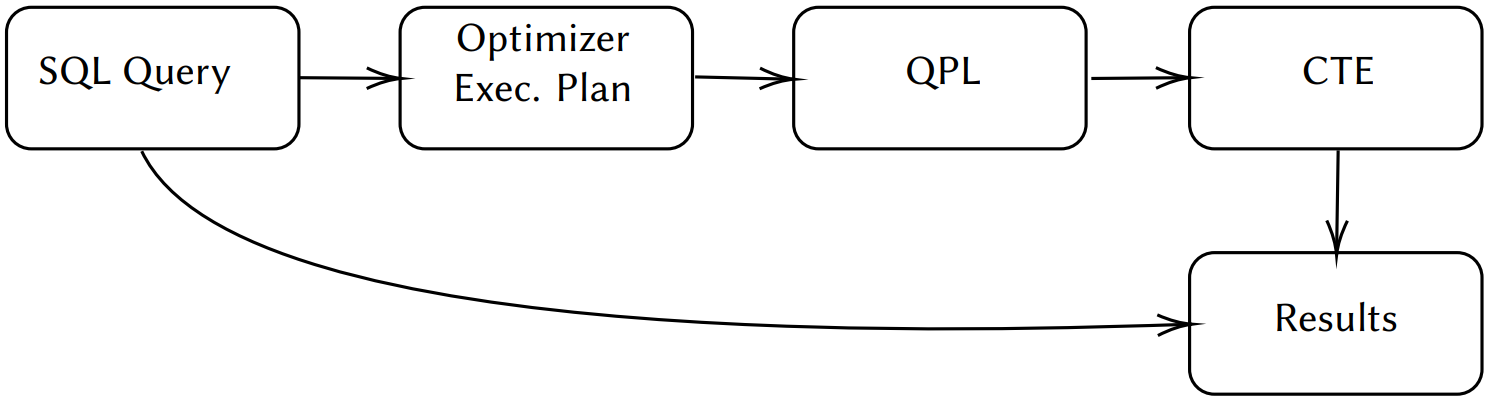
\includegraphics[width=\textwidth]{qpl-creation.png}
    \end{center}
\end{frame}

\section{Experiments and Results}

\begin{frame}{Experimental Setup}
    \begin{itemize}
        \item We evaluate a direct QPL prediction model on the development set of Spider
        \item Our baselines are:
        \begin{itemize}
            \item NatSQL + RAT -- uses a syntactic transformation on the query to learn a version of SQL that is more aligned with natural language syntax.
            \item T5-3B + PICARD -- generates an SQL query using a fine-tuned T5-3B model and makes sure the SQL is syntactically valid using the PICARD method
            \item DIN-SQL -- uses various prompting techniques with GPT-4
            \item GPT-3.5 Turbo -- uses a 5-shot prompt
        \end{itemize}
    \end{itemize}
\end{frame}

\begin{frame}{PICARD Constrained Decoding for QPL}
    \begin{itemize}
        \item PICARD is a constrained decoding method
        \item Without retraining a model, PICARD ``plugs'' on top of an existing auto-regressive model and operates at inference time
        \item During beam search, the beams are sent to an incremental parser which decides whether the current parse together with the candidate token still make a valid SQL query prefix
        \item Significantly reduces number of syntactically invalid SQL, and can be made to work with other languages as well, not just SQL
        \item We adapted Picard to QPL by writing an incremental parser for QPL
    \end{itemize}
    \tiny{Scholak, Schucher and  Bahdanau, \textit{PICARD: Parsing Incrementally for Constrained Auto-Regressive Decoding from Language Models}, EMNLP 2021}
\end{frame}

\begin{frame}{Direct Prediction of SQL vs. QPL (No Values)}
    \begin{table}[h]
    \centering
    \begin{tabular}{lrrrr}
    \toprule
    Spider Difficulty & Q $\rightarrow$ QPL & T5-3B + PICARD & Support \\ \midrule
    Easy        & 87.5\%  & 91.9\% & 248  \\
    Medium      & 84.3\%  & 76.9\% & 446  \\
    Hard        & 66.7\%  & 64.9\% & 174  \\
    Extra Hard  & \alert{\textbf{54.8\%}}  & 44.6\% & 166  \\
    \midrule
    Overall & \textbf{77.4\%} & 73.3\% & 1034 \\
    \bottomrule
    \end{tabular}
    \end{table}

    \begin{itemize}
        \item All other things being equal, QPL is easier to learn than SQL for neural architecture.
        \item Most significant gain on \alert{complex queries}
    \end{itemize}
\end{frame}

\begin{frame}{Direct Prediction of SQL vs. QPL (with Values)}
    \begin{table}[h]
    \centering
    \begin{tabular}{lrrrr}
    \toprule
    Spider Difficulty & Q $\rightarrow$ QPL & T5-3B + PICARD & Support \\ \midrule
    Easy	    & 93.5\%  & 91.5\% & 248  \\
    Medium	    & 89.0\%  & 88.3\% & 446  \\
    Hard	    & 74.7\%  & 69.5\% & 174  \\
    Extra Hard	& 65.1\%  & 63.9\% & 166  \\
    \midrule
    Overall	    & \textbf{83.8\%}  & 82.0\% & 1034 \\
    \bottomrule
    \end{tabular}
    \end{table}

    \begin{itemize}
        \item All other things being equal, QPL is easier to learn than SQL for neural architecture.
        \item Most significant gain on \alert{complex queries}
    \end{itemize}
\end{frame}

\begin{frame}{QPL is also Easier for Humans to Read}
    \begin{table}[h]
    @@@ Summarize here how many of these are "correct judgments" / "incorrect judgments"
    @@@ Relate this to RQ2
    \centering
    \begin{tabular}{llc}
        \toprule
        \textbf{Type} & \textbf{Gold label} & \textbf{Correct} \\
        \midrule
        QPL & Incorrect query   & 53\% \\
            & Correct query     & 79\% \\
         &                      & \textbf{67\%} \\
        \midrule
        SQL & Incorrect query  & 50\% \\
            & Correct query    & 25\% \\
         &           & \textbf{34\%} \\
        \bottomrule
    \end{tabular}
\end{table}
\end{frame}

\section{Conclusion and Future Work}

\begin{frame}{Conclusion and Future Work}
    \begin{itemize}
        \item Both humans and language models have an easier time understanding QPL than SQL for complex queries
        \item Even with capable LLMs such as GPT-4, the problem of making SQL more accessible to non-experts is still an open problem
    \end{itemize}
\end{frame}

\begin{frame}{The Quest for Modularity}
    \begin{itemize}
        \item In this work, we just replaced SQL with a more modular data retrieval language.
        \item In current work, we aim to take advantage of QPL's modularity to improve the learning process to increase the explainability of the resulting model.
        \begin{enumerate}
        \item \textbf{Auto-regressive model}: given a Question and the first steps of a QPL, predict the next step.
        \item \textbf{Data augmentation}: synthesize new (Question, QPL) pairs by composing smaller QPLs into larger ones and synthesizing a question.
        \item \textbf{Multi-turn}: specifying the desired data in a single natural question is complex - multi-turn conversational refinement of questions and predicted QPL.
        \item \textbf{Planning vs. Low-level}: disentangle knowledge for planning complex data retrieval operations given a relational schema and implementing small computational steps.
        \end{enumerate}
    \end{itemize}
\end{frame}

\begin{frame}[fragile]{Question Decomposition}
    \begin{minted}[fontsize=\scriptsize]{text}
Schema:
Table Visitor (ID, Name, Age, Level_of_membership)
Table Museum (Museum_ID, Name, Open_Year, Num_of_staff)
Table Visit (Visitor_ID, Museum_ID, Total_Spent, Num_of_Ticket)

Question:
What is the total ticket expense of the visitors whose membership level is 1?

QPL Plan:
#1 = Scan Table [ visitor ] Predicate [ Level_of_membership = 1 ] Output [ ID ]
#2 = Scan Table [ visit ] Output [ visitor_ID , Total_spent ]
#3 = Join [ #1, #2 ] Predicate [ #1.ID = #2.visitor_ID ] Output [ #2.Total_spent ]
#4 = Aggregate [ #3 ] Output [ SUM(Total_spent) AS Sum_Total_spent ]

Natural Language Plan:
#1 = Scan the table Visitor to find who are the visitors with membership level 1
#2 = Scan the table Visit to find what is the total spent by visitors during their visits
#3 = Join #1 and #2 to find what is the total spent by each visitor with
     membership level 1 during their visits
#4 = Group #3 by Visitor and aggregate the sum of total spent to find what is the
     total spent by all visitors with membership level 1 during their visit
    \end{minted}
\end{frame}

\end{document}